\documentclass{article}
\usepackage{a4wide}
\usepackage{graphicx}

\begin{document}

\section*{A Developers Guide to Earth Plugins}

\subsection*{What do I need to know before I develop a plugin for Earth?}

The following are the pre-requisites for developing a plugin for Earth:

\begin{itemize}
   \item Ruby - the language
   \item Rails - the fundamentals of the framework
   \item Earth - installed on a server some where
\end{itemize} 

%Besides them, you will also need to keep the API specifications handy for reference. 

\subsection*{Right, I got all of them, what do I do now?}

One word- ``code''.

Every Earth plugin must contain the following lines of codes:

\begin{figure}[h]
   \centering
   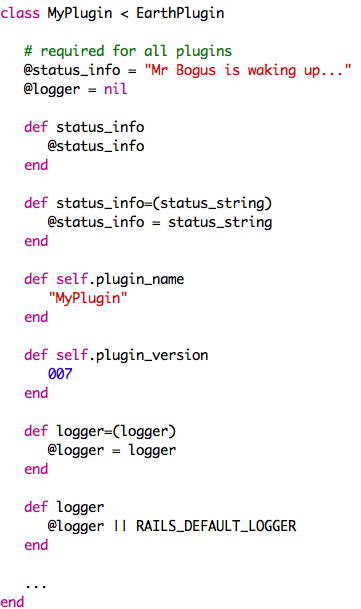
\includegraphics[scale=0.5]{plugin_standard_codes.png}
\end{figure}

The following are the description for each standard methods:

\begin{itemize}
   \item \textbf{\texttt{status\_info}} These methods are accessors to the status of the plugin to be reported back to the daemon. The one with an ``='' sign is to set the status info. 
   \item \textbf{\texttt{self.plugin\_name}} The name of the plugin. It must be the same as name used during installation. 
   \item \textbf{\texttt{self.plugin\_version}} The version of the plugin. It must be the same as the version used during installation. 
   \item \textbf{\texttt{logger}} These methods are accessors to the daemon's log file writer. It allows the plugin to write to the daemon's logger. 
\end{itemize}

After this, it is your own codes. 

\subsection*{I have finished my plugin, how do I install and test?}

Sorry, please stay tuned. The installation flow has not been established yet. 


\end{document}  